\vspace{-0.2cm}
\section{Introduction}
\label{sec:prime_intro}
\vspace{-0.2cm}
%% motivation, brief description of the problem statement
The death of Moore's Law~\citep{esmaeilzadeh2011dark} has driven the growth of specialized hardware accelerators. These specialized accelerators are tailored to specific applications~\citep{yazdanbakhsh2021apollo,reagen2017case,prac_dse:mascots:2019,shi2020learned}. To design specialized accelerators, akin to standard online RL, designers first spend considerable amounts of time developing simulators that closely model the real accelerator performance, and then optimize the accelerator using the simulator. While such simulators can automate accelerator design, this requires a large number of simulator queries for each new design, both in terms of simulation time and compute requirements, and this cost increases with the size of the design space~\citep{yazdanbakhsh2021evaluation,shi2020learned,hegdemind}.
Moreover, most of the accelerators in the design space are typically infeasible~\citep{hegdemind,yazdanbakhsh2021apollo} because of build errors in silicon or compilation/mapping failures. 
When the target applications change or a new application is added, the complete simulation-driven procedure is generally repeated.
To make such approaches efficient and practically viable, designers typically ``bake-in'' constraints or otherwise narrow the search space, but such constraints can leave out high-performing solutions~\citep{dmazerunner,timeloop,marvel}.

%% Transition to the new paradigm, define data-driven stuff, etc
An alternate approach, proposed in this chapter, is to devise an \textit{offline} optimization method, based on offline RL techniques, that only utilizes a database of previously tested accelerator designs, annotated with measured performance metrics, to produce new optimized designs \emph{without} additional active queries to an explicit silicon or a cycle-accurate simulator. In the context of hardware accelerator design, such an offline approach provides three key benefits: \textbf{(1)} it significantly shortens the recurring cost of running large-scale simulation sweeps, \textbf{(2)} it alleviates the need to explicitly bake in domain knowledge or search space pruning, and {\textbf{(3)} it enables data re-use by empowering the designer to optimize accelerators for new unseen applications, by the virtue of effective generalization.}
While data-driven approaches have shown promising results in biology~\citep{fu2021offline,brookes19a,trabucco2021conservative},
using offline optimization methods to design accelerators has been challenging primarily due to the abundance of infeasible design points~\citep{yazdanbakhsh2021apollo,hegdemind}.

%% The key idea of our method
The key contribution of this chapter is \primemethodname\,, a conservative value-based approach to automatically architect high-performing application-specific accelerators by using only previously collected static data. Since the problem of accelerator design requires us to only select one action, and not a sequence of actions, we do not need to learn a complete value function. Instead, it suffices for \primemethodname\ to learn a conservative model of the one-step reward or objective function from the offline dataset (e.g., latency or power consumption of an accelerator).
Then, \primemethodname\ finds high-performing application-specific accelerators by optimizing the architectural parameters against this learned conservative model, as shown in Figure~\ref{fig:prime_overview}. Akin to the full sequential setting, while optimizing na\"ively trained
\begin{figure}[t!]
    \centering
    \vspace{-0.1cm}
    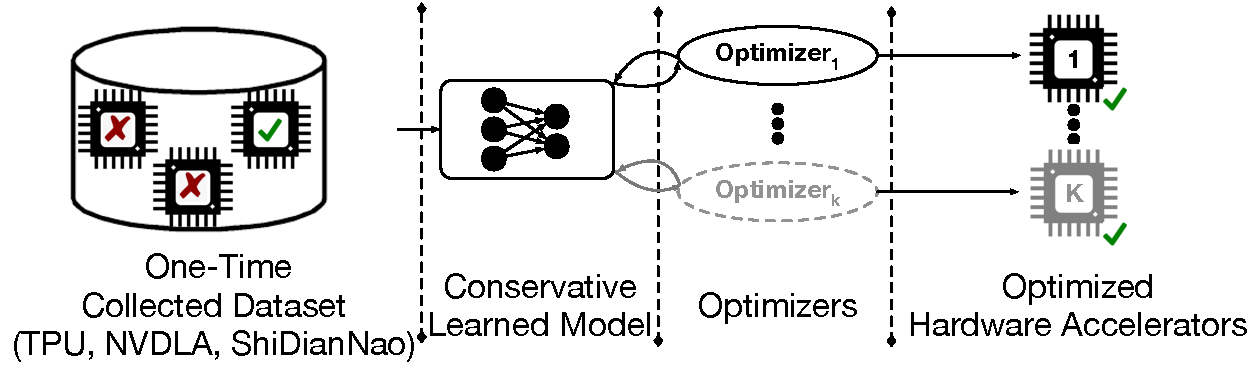
\includegraphics[width=0.8\linewidth]{chapters/prime/figs/overview/prime-overview.pdf}
    \vspace{-0.2cm}
    \caption{\footnotesize{\textbf{Overview of \primemethodname.} We use a one-time collected dataset of prior accelerator designs, including TPU-style~\citep{yazdanbakhsh2021evaluation}, NVDLA-style~\citep{nvdla}, and ShiDianNao-style~\citep{shidiannao} accelerators to train a conservative surrogate model, which is used to design accelerators to meet desired goals and constraints.}}
    \vspace{-0.4cm}
    \label{fig:prime_overview}
\end{figure}
models of the objective function usually produces poor-performing, out-of-distribution designs that erroneously appear optimistic~\citep{kumar2019model,brookes19a,trabucco2021conservative},
the conservative model in \primemethodname\ gives rise to good designs. Furthermore, in contrast to prior works that discard infeasible points~\citep{hegdemind,trabucco2021conservative}, our proposed method instead incorporates infeasible points when learning the conservative surrogate model by treating them as additional negative samples. During evaluation, \primemethodname\ optimizes the learned conservative model.

Our results show that \primemethodname\ architects hardware accelerators that improve over the best design in the training dataset, on average, by 2.46$\times$ (up to 6.7$\times$) when specializing for a single application. 
%
In this case, \primemethodname\ also improves over the best conventional simulator-driven optimization methods by 1.54$\times$ (up to 6.6$\times$).
%
These performance improvements are obtained while reducing the total simulation time to merely 7\% and 1\% of that of the simulator-driven methods for single-task and multi-task optimization, respectively.
%
More importantly, a contextual version of \primemethodname\ can design accelerators that are \emph{jointly optimal} for a set of \textit{nine} applications without requiring any additional domain information.
%
In this challenging setting, \primemethodname\ improves over simulator-driven methods, which tend to scale poorly as more applications are added, by 1.38$\times$.
%
Finally, we show that the models trained with \primemethodname\ on a set of training applications can be readily used to obtain accelerators for \textit{unseen} target applications, without any retraining on the new application.
%
Even in this \emph{zero-shot} optimization scenario, \primemethodname\ outperforms simulator-based methods that require re-training and active simulation queries by up to 1.67$\times$.
%
In summary, \primemethodname\ allows us to effectively address the shortcomings of simulation-driven approaches, it: (1) significantly reduces the simulation time, (2) enables data reuse and enjoys generalization properties, and (3) does not require domain-specific engineering or search space pruning.
%
